\documentclass[conference]{IEEEtran}

\usepackage{amsmath}
\usepackage{graphicx}
\usepackage{booktabs}
\usepackage{cite}
\usepackage{url}
\usepackage{tikz}
\usepackage{pgfplots}
\usetikzlibrary{arrows.meta,positioning}
\pgfplotsset{compat=1.18}
\graphicspath{{figures/}}

\title{Grid-Aware Demand Clustering for Electric Vehicle Charging Station Siting and Sizing: A London Case Study}

\author{
\IEEEauthorblockN{Author Name}
\IEEEauthorblockA{Department or Institution\\
Email: author@example.com}
}

\begin{document}

\maketitle

\begin{abstract}
The planning of public electric vehicle (EV) charging infrastructure in dense cities must balance user convenience, demand coverage, investment cost, and the ability of the local electricity network to accommodate additional charging load. Many siting studies optimise candidate stations after demand points have already been grouped geographically, which can delay the consideration of grid-side constraints until a late planning stage. This paper proposes Grid-aware Demand Clustering for Location-Capacity Optimisation (GDC-LCO), a grid-aware framework for EV charging station siting and sizing. The method first partitions an urban study area into charging service zones using spatial location, demand intensity, transport accessibility, and a reproducible grid-risk proxy. It then performs location-capacity optimisation within each service zone. A London Borough of Barnet case study is developed using OpenStreetMap features from Overpass, including charging stations, parking locations, points of interest, major roads, residential land use, substations, and an administrative boundary. Results show that the proposed grid-aware method reduces grid impact per installed charger relative to geographical and demand-weighted clustering while maintaining high demand coverage. The findings indicate that grid-aware clustering should be interpreted as a trade-off tool rather than a universally distance-minimising method.
\end{abstract}

\begin{IEEEkeywords}
Electric vehicle charging stations, siting and sizing, demand clustering, grid-aware planning, urban infrastructure planning.
\end{IEEEkeywords}

\section{Introduction and Literature Review}

The rapid adoption of electric vehicles creates increasing pressure on public charging infrastructure in dense urban areas. Charging demand is spatially uneven because it is shaped by residential density, workplace and commercial activity, road accessibility, parking availability, and the distribution of existing charging facilities. Planning charging stations therefore requires more than minimising geographical distance between users and stations.

Urban electric vehicle charging station planning faces three related challenges. First, demand varies substantially across neighbourhoods and times of day. Second, city-scale siting and sizing can become computationally expensive when many demand points and candidate sites are considered simultaneously. Third, many planning approaches focus primarily on demand coverage and user convenience, while grid-side connection cost, hosting capacity, or peak-load pressure are considered only after candidate locations have been generated.

Existing studies on charging demand modelling commonly use travel surveys, population density, land use, points of interest, traffic flow, and charging transaction data to estimate spatial demand. Siting and sizing studies have formulated variants of covering, p-median, mixed-integer optimisation, and multi-objective models to balance distance, cost, coverage, and utilisation. Clustering-based infrastructure planning has also been used to partition large urban problems into smaller service regions. However, clustering stages are often based on geography alone or demand-weighted geography. Grid-aware planning studies, by contrast, usually introduce distribution network constraints or hosting-capacity limits at the optimisation stage rather than embedding grid-related information into service-zone formation.

This paper addresses the gap by proposing a grid-aware demand clustering framework for electric vehicle charging station planning. The core idea is to use clustering as a problem decomposition tool, not as the final siting decision. Demand points are first partitioned into service zones using spatial location, charging demand, transport accessibility, and grid-risk proxy features. Candidate charging stations are then selected and sized within each service zone.

The contributions of this paper are threefold:
\begin{itemize}
  \item A grid-aware demand clustering method is proposed for interpretable electric vehicle charging service-zone partitioning.
  \item A location-capacity optimisation framework is developed to jointly consider user service distance, investment cost, capacity adequacy, and grid impact.
  \item A reproducible London case-study pipeline is designed with baseline comparison, sensitivity analysis, and open-source research code.
\end{itemize}

\section{Problem Formulation}

Let \(I\) denote the set of charging demand points and \(J\) denote the set of candidate charging station sites. Each demand point \(i \in I\) has a location, charging demand weight \(D_i\), accessibility score \(A_i\), and grid-risk proxy \(G_i\). Each candidate site \(j \in J\) has a location, fixed construction cost, charger installation cost, grid-risk score, and maximum charger capacity.

The main decision variables are:
\begin{align}
y_j &= \begin{cases}1, & \text{if candidate site } j \text{ is selected}\\0, & \text{otherwise,}\end{cases}\\
n_j &= \text{number of chargers installed at site } j,\\
x_{ij} &= \begin{cases}1, & \text{if demand point } i \text{ is assigned to site } j\\0, & \text{otherwise.}\end{cases}
\end{align}

The general objective is formulated as:
\begin{equation}
\min F = w_1 F_{\text{distance}} + w_2 F_{\text{investment}} + w_3 F_{\text{grid}} + w_4 F_{\text{capacity}}.
\end{equation}

The distance component is:
\begin{equation}
F_{\text{distance}} = \sum_{i \in I}\sum_{j \in J} D_i d_{ij} x_{ij},
\end{equation}
where \(d_{ij}\) is the travel or spatial distance between demand point \(i\) and station \(j\).

The investment component is:
\begin{equation}
F_{\text{investment}} = \sum_{j \in J} c_j^{\text{fixed}} y_j + c^{\text{charger}}_j n_j.
\end{equation}

The grid impact component is represented using a proxy:
\begin{equation}
F_{\text{grid}} = \sum_{j \in J} P_j G_j,
\end{equation}
where \(P_j\) is the installed charging power at site \(j\).

The capacity penalty is:
\begin{equation}
F_{\text{capacity}} = \sum_{j \in J} \max(0, Q_j - C_j),
\end{equation}
where \(Q_j\) is assigned demand and \(C_j\) is installed station capacity.

\section{Proposed Grid-Aware Demand Clustering for Location-Capacity Optimisation Methodology}

The proposed Grid-aware Demand Clustering for Location-Capacity Optimisation (GDC-LCO) framework consists of demand feature construction, grid-risk proxy construction, service-zone clustering, candidate station generation, and location-capacity optimisation.

\begin{figure*}[!t]
\centering
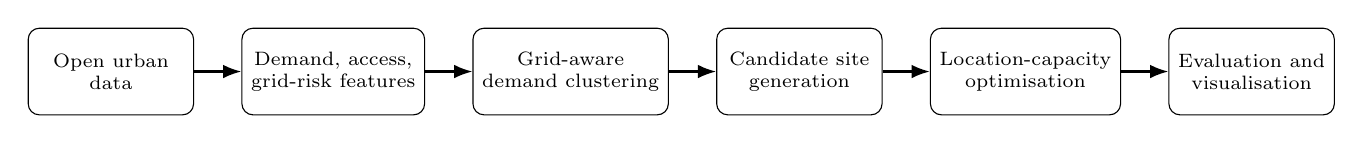
\begin{tikzpicture}[
node distance=6mm,
box/.style={draw, rounded corners, align=center, minimum width=21mm, minimum height=11mm, font=\scriptsize},
arrow/.style={-Latex, thick}
]
\node[box] (data) {Open urban\\data};
\node[box, right=of data] (features) {Demand, access,\\grid-risk features};
\node[box, right=of features] (cluster) {Grid-aware\\demand clustering};
\node[box, right=of cluster] (candidate) {Candidate site\\generation};
\node[box, right=of candidate] (optimise) {Location-capacity\\optimisation};
\node[box, right=of optimise] (eval) {Evaluation and\\visualisation};
\draw[arrow] (data) -- (features);
\draw[arrow] (features) -- (cluster);
\draw[arrow] (cluster) -- (candidate);
\draw[arrow] (candidate) -- (optimise);
\draw[arrow] (optimise) -- (eval);
\end{tikzpicture}

\caption{Workflow of the proposed GDC-LCO framework. Urban open data are transformed into demand, accessibility, and grid-risk features. These features are used to form service zones before candidate site selection, station sizing, and evaluation.}
\label{fig:method_flowchart}
\end{figure*}

\subsection{Demand Feature Construction}
Charging demand is represented as a weighted combination of residential, commercial, and road-related components:
\begin{equation}
D_i = \alpha D_i^{\text{res}} + \beta D_i^{\text{com}} + \gamma D_i^{\text{road}}.
\end{equation}

\subsection{Grid-Risk Proxy Construction}
In the absence of full distribution network topology, grid impact is represented by reproducible proxy variables such as peak-load pressure, assumed hosting capacity, existing charging density, or distance to an assumed connection point. A simple proxy can be expressed as:
\begin{equation}
G_i = \frac{\text{peak load proxy}_i}{\text{hosting capacity proxy}_i}.
\end{equation}

\subsection{Clustering Methods}
Three clustering methods are compared. Geographical K-means uses only spatial coordinates. Demand-weighted K-means uses demand weights when updating cluster centroids. The proposed grid-aware demand clustering uses:
\begin{equation}
z_i = [\lambda_s lon_i, \lambda_s lat_i, \lambda_d D_i, \lambda_a A_i, \lambda_g G_i].
\end{equation}

\subsection{Location-Capacity Optimisation Within Clusters}
After clustering, each service zone is optimised independently. This decomposition reduces the effective problem size and produces interpretable local planning regions. The current research code implements a lightweight greedy solver to maintain reproducibility without proprietary optimisation software, while the documented formulation supports later replacement with a mixed-integer or multi-objective optimiser.

\subsection{Algorithm Summary}
\begin{enumerate}
  \item Construct demand, accessibility, and grid-risk features.
  \item Partition demand points using grid-aware clustering.
  \item Generate candidate stations within each service zone.
  \item Select stations and charger capacities inside each zone.
  \item Aggregate selected stations and evaluate distance, cost, coverage, grid impact, and utilisation.
\end{enumerate}

\section{Case Study and Experimental Setup}

The target case study is London, with Barnet or selected Inner London boroughs as the initial implementation area. London is suitable because it provides rich open urban data, a dense and heterogeneous charging environment, and a relevant policy context for public charging infrastructure planning.

The MVP first validates the full pipeline on a synthetic London-like dataset. The synthetic case generates demand points, candidate sites, existing stations, accessibility scores, hosting-capacity proxies, and grid-risk scores from reproducible random seeds. This allows the methodology, code structure, metrics, and visualisation outputs to be tested before real data integration.

The planned real-data sources include public charging station locations, population density, points of interest, road network data, borough boundaries, parking or residential density proxies, and grid-risk proxy variables. All real-data integration will be handled through configuration files and data loaders so that the core algorithms remain city-agnostic.

The experimental comparison includes geographical K-means, demand-weighted K-means, and the proposed grid-aware demand clustering method. The main evaluation metrics are average service distance, demand coverage ratio, investment cost, grid impact score, utilisation balance, unserved demand, selected station count, installed chargers, and computation time.

\section{Results and Discussion}

This section will report the spatial demand distribution, clustering service zones, selected charging station sites, installed charger capacities, and comparison results across baseline methods.

The expected analysis is organised around five questions:
\begin{enumerate}
  \item How does charging demand vary across the study area?
  \item How do geographical, demand-weighted, and grid-aware clusters differ spatially?
  \item Where are charging stations selected and how much capacity is installed?
  \item What trade-offs appear among service distance, investment cost, coverage, grid impact, and utilisation?
  \item How sensitive are the results to the number of clusters and grid-risk feature weight?
\end{enumerate}

The key claim is not that the proposed method always minimises service distance. Instead, the method is expected to provide a more balanced planning outcome by explicitly considering grid-risk information during service-zone partitioning.

\section{Conclusion}

This paper proposes a grid-aware demand clustering framework for electric vehicle charging station siting and sizing. The framework uses clustering to decompose city-scale planning into interpretable service zones and then performs location-capacity optimisation within each zone.

Future work will integrate real distribution network topology, power-flow constraints, dynamic charging demand, queueing models, multi-objective optimisation, and cross-city validation.


\bibliographystyle{IEEEtran}
\bibliography{references}

\end{document}
